%prop algorithm methods
To correct for the effect of the bright spots in the image being over bright and the high-key appearance resulting from all the shadows being brightened, we used an algorithm that maps the black and white points of the image to the same value, and adjusts the colours in between to match the target average colour.

\begin{algorithm}[H]
\caption{Proportional adjustment relative to average color}
\label{eq:prop_algo}
\begin{algorithmic}
\State $\mean{C_T} \gets \Call{Mean}{\vect{C_T}(U)}$
\State $\mean{C_S} \gets \Call{Mean}{\vect{C_S}(V)}$
\For{each pixel $i \in S$}
\If{$\vect{C_S}(i) \leq \mean{C_S}$}
\State $\vect{C_O}(i) \gets \displaystyle \left(\frac{\mean{C_T}}{\mean{C_S}}\right)\vect{C_S}(i)$
\Else
\State $\vect{C_O}(i) \gets \displaystyle 255 - \left(\frac{255 - \mean{C_T}}{255 - \mean{C_S}}\right)(255 - \vect{C_S}(i))$
\EndIf
\EndFor
\end{algorithmic}
\end{algorithm}

In Table \ref{tab:prop_test} we show the results for colour transfers between all possible combinations of our test images.
\begin{longtable}{|N||c|c|c|}
	\caption{Test results of brightening proportionally based on distance of color to the average.\label{tab:prop_test}}\\
	\hline
	\multicolumn{1}{|c||}{No.} & Original & Target & Results \\ 
	\hline
	    \label{row:prop_test_1} &
  \begin{minipage}{.29\textwidth}
    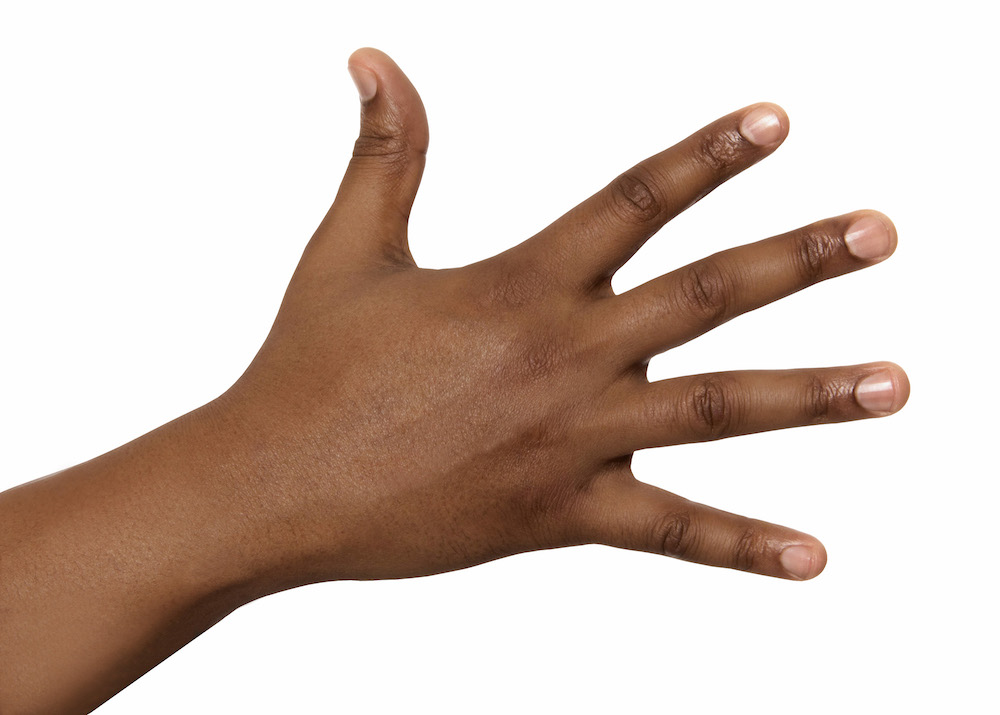
\includegraphics[width=\textwidth,height=\textheight,keepaspectratio]{../inputs/hand_dark.jpg}
  \end{minipage} & 
  \begin{minipage}{.29\textwidth}
    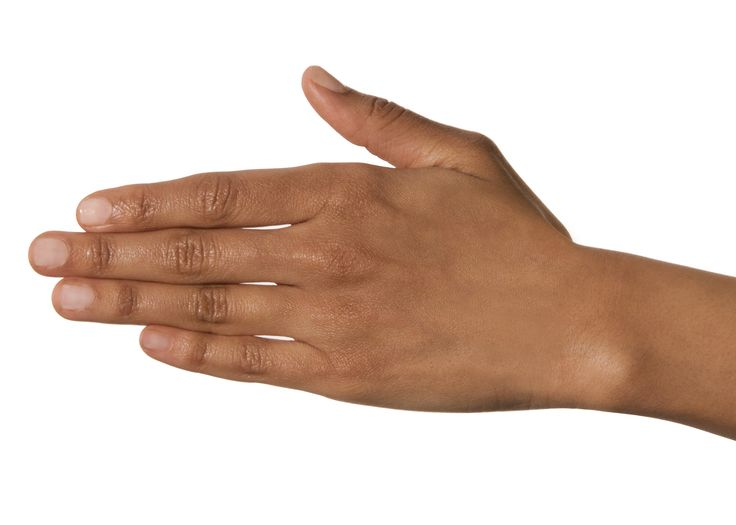
\includegraphics[width=\textwidth,height=\textheight,keepaspectratio]{../inputs/hand_brown.jpg}
  \end{minipage} & 
  \begin{minipage}{.29\textwidth}
    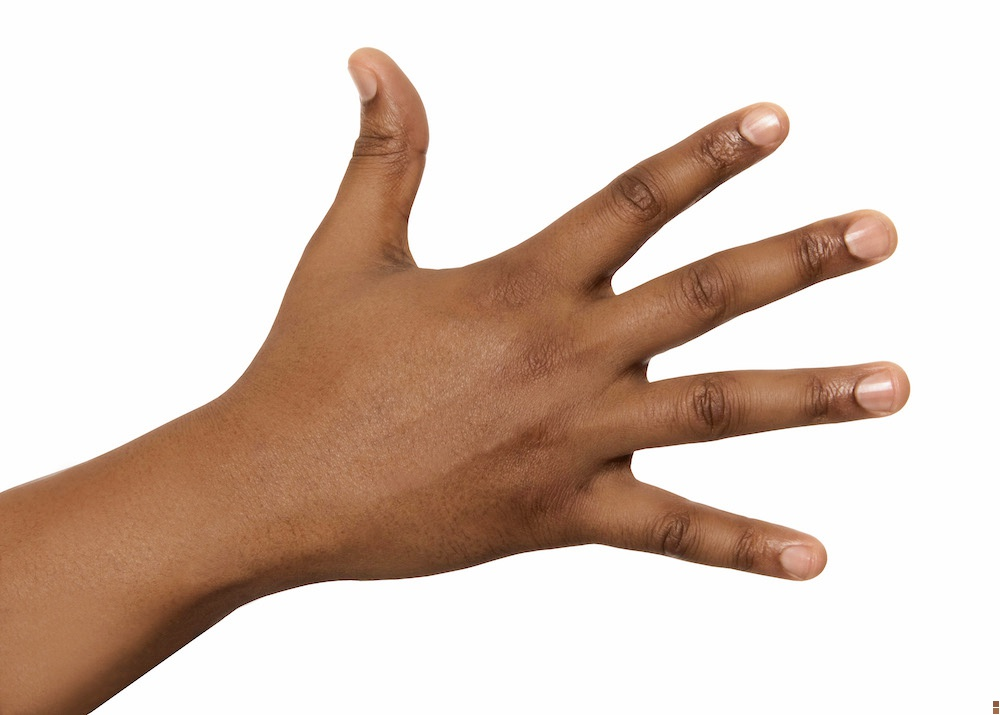
\includegraphics[width=\textwidth,height=\textheight,keepaspectratio]{../rc_test/outputs/20170516_proportional_test/hand_dark_to_hand_brown.jpg}
  \end{minipage} \\
\hline  \label{row:prop_test_1} &
  \begin{minipage}{.29\textwidth}
    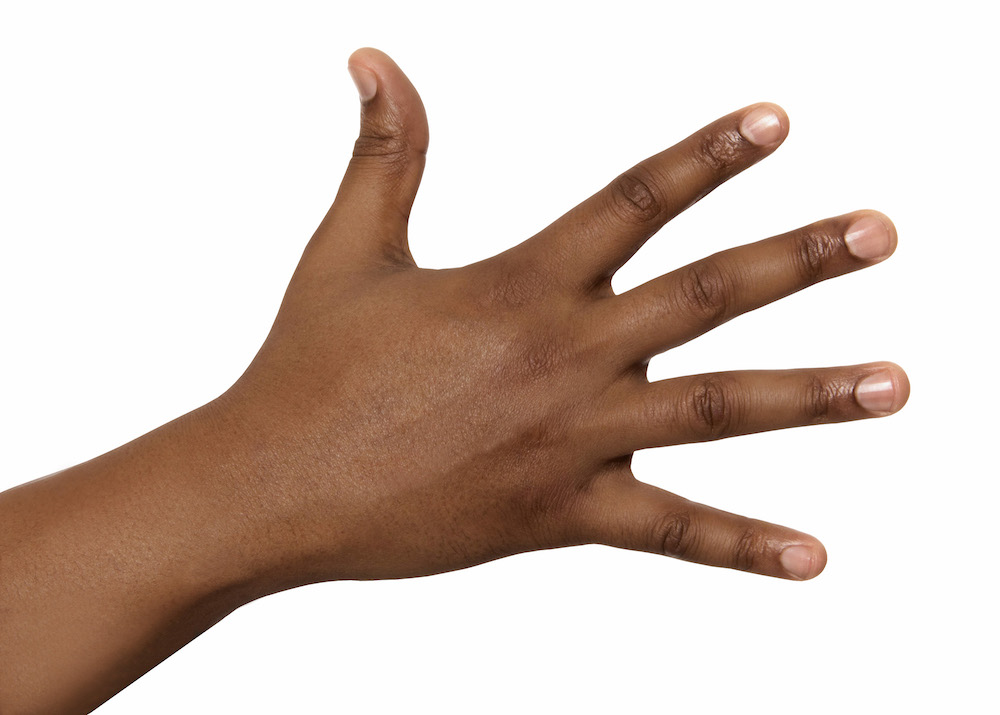
\includegraphics[width=\textwidth,height=\textheight,keepaspectratio]{../inputs/hand_dark.jpg}
  \end{minipage} & 
  \begin{minipage}{.29\textwidth}
    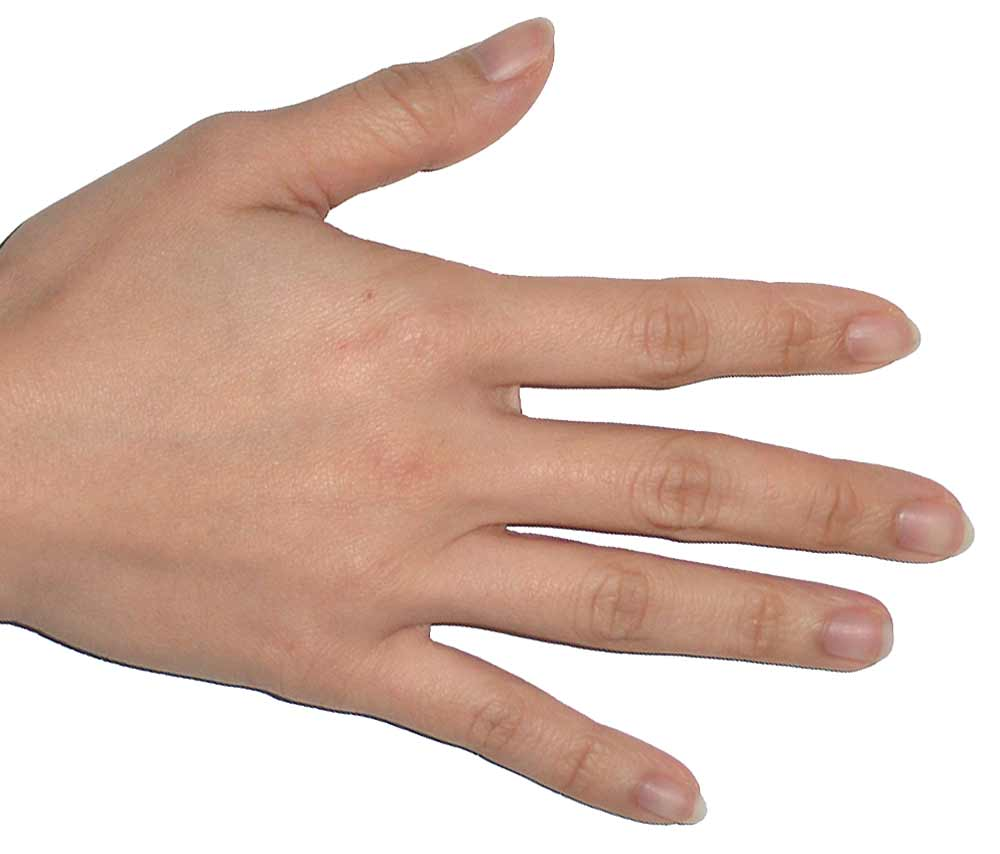
\includegraphics[width=\textwidth,height=\textheight,keepaspectratio]{../inputs/hand_light.jpg}
  \end{minipage} & 
  \begin{minipage}{.29\textwidth}
    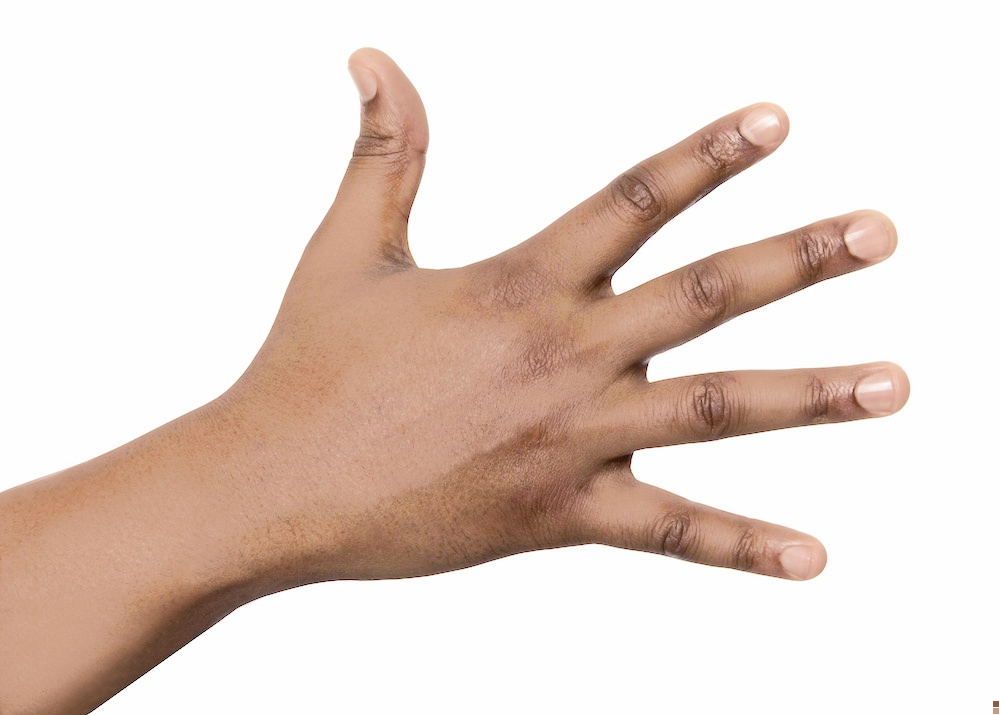
\includegraphics[width=\textwidth,height=\textheight,keepaspectratio]{../rc_test/outputs/20170516_proportional_test/hand_dark_to_hand_light.jpg}
  \end{minipage} \\
\hline  \label{row:prop_test_1} &
  \begin{minipage}{.29\textwidth}
    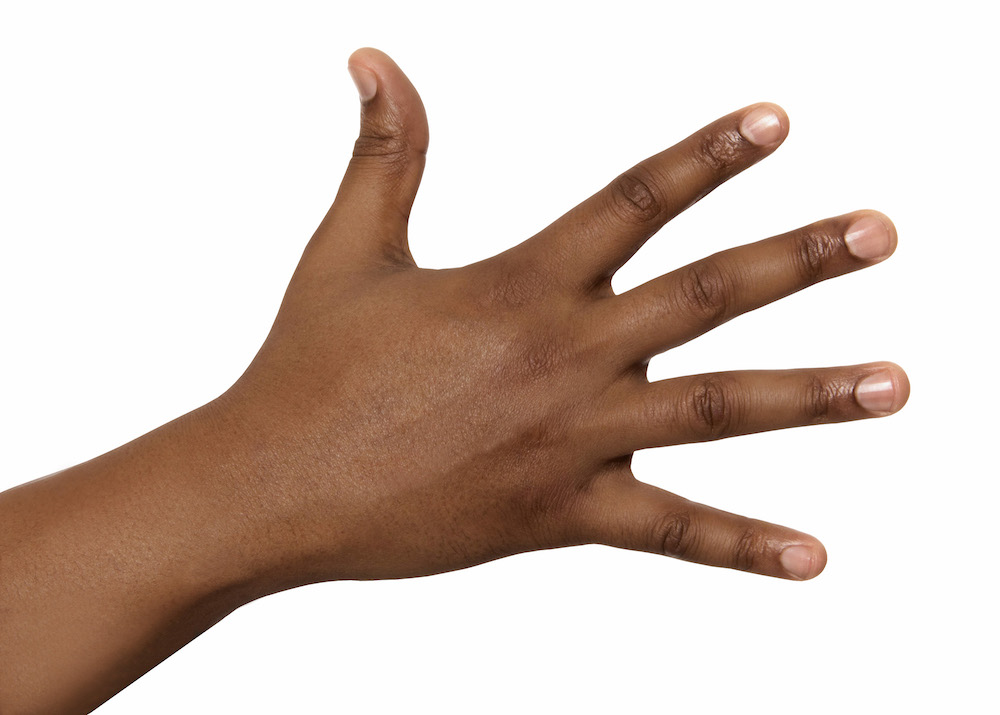
\includegraphics[width=\textwidth,height=\textheight,keepaspectratio]{../inputs/hand_dark.jpg}
  \end{minipage} & 
  \begin{minipage}{.29\textwidth}
    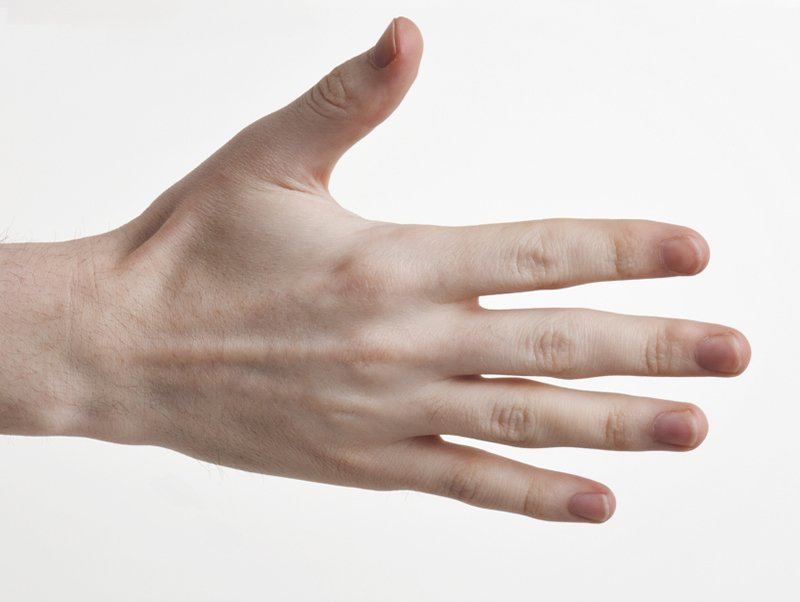
\includegraphics[width=\textwidth,height=\textheight,keepaspectratio]{../inputs/hand_pale.jpg}
  \end{minipage} & 
  \begin{minipage}{.29\textwidth}
    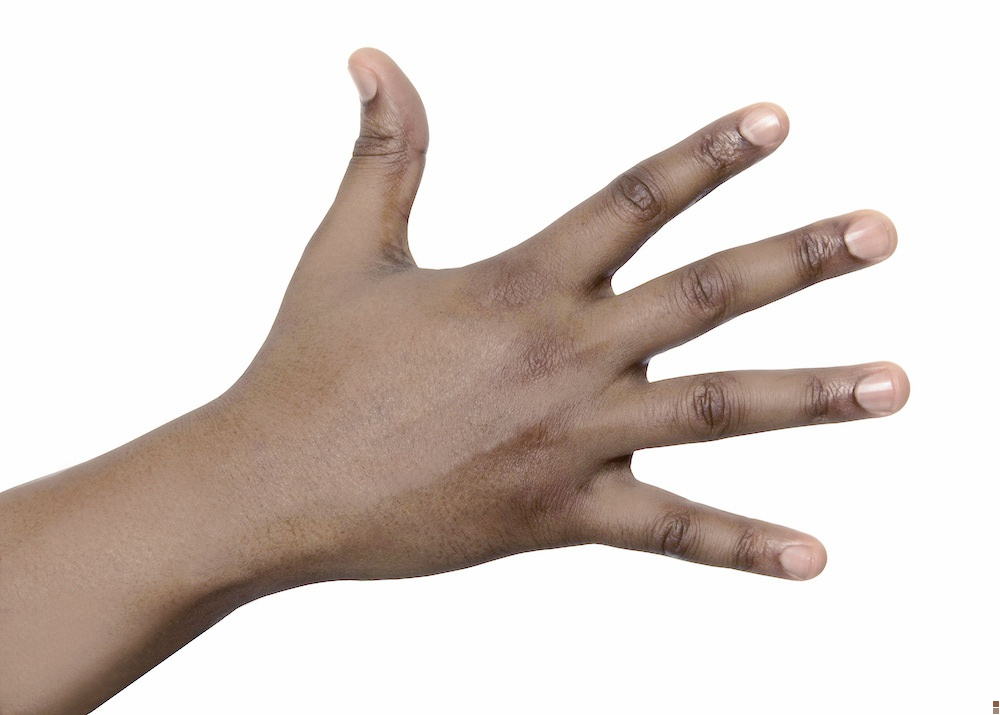
\includegraphics[width=\textwidth,height=\textheight,keepaspectratio]{../rc_test/outputs/20170516_proportional_test/hand_dark_to_hand_pale.jpg}
  \end{minipage} \\
\hline  \label{row:prop_test_1} &
  \begin{minipage}{.29\textwidth}
    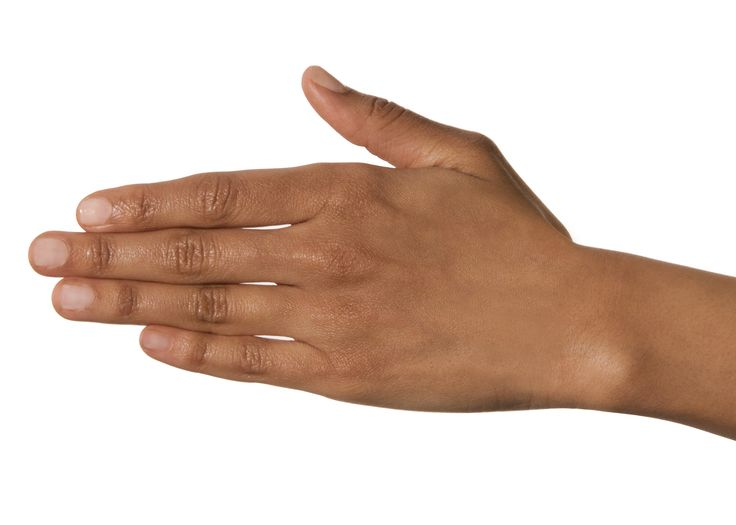
\includegraphics[width=\textwidth,height=\textheight,keepaspectratio]{../inputs/hand_brown.jpg}
  \end{minipage} & 
  \begin{minipage}{.29\textwidth}
    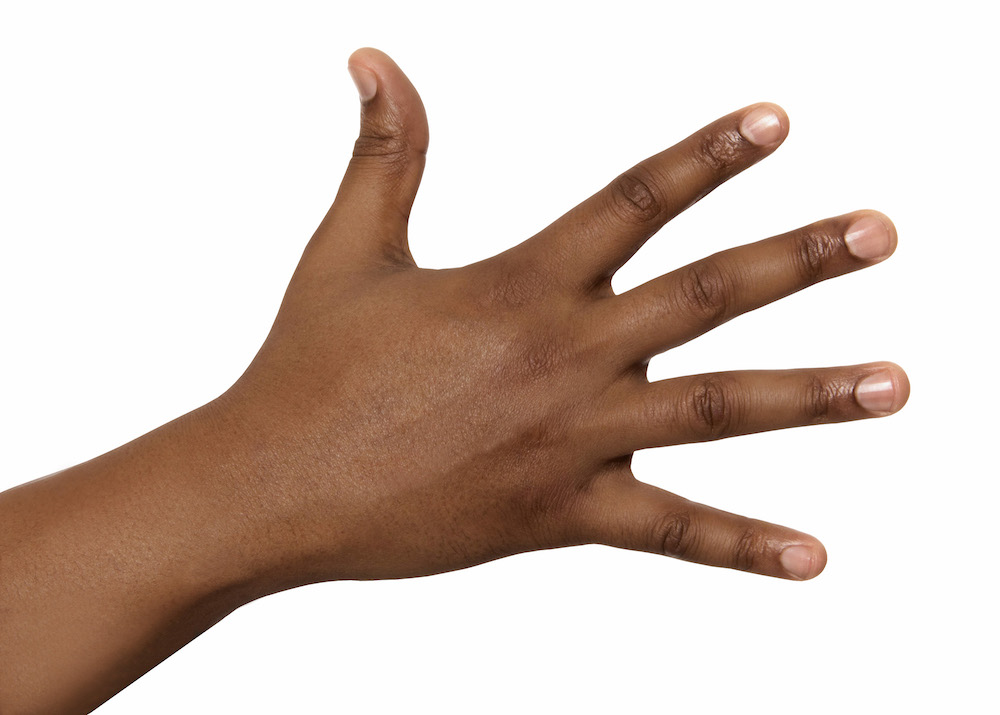
\includegraphics[width=\textwidth,height=\textheight,keepaspectratio]{../inputs/hand_dark.jpg}
  \end{minipage} & 
  \begin{minipage}{.29\textwidth}
    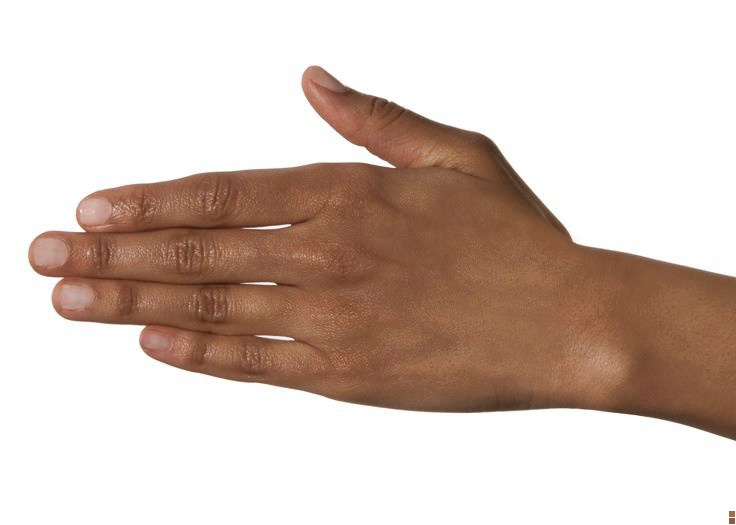
\includegraphics[width=\textwidth,height=\textheight,keepaspectratio]{../rc_test/outputs/20170516_proportional_test/hand_brown_to_hand_dark.jpg}
  \end{minipage} \\
\hline  \label{row:prop_test_1} &
  \begin{minipage}{.29\textwidth}
    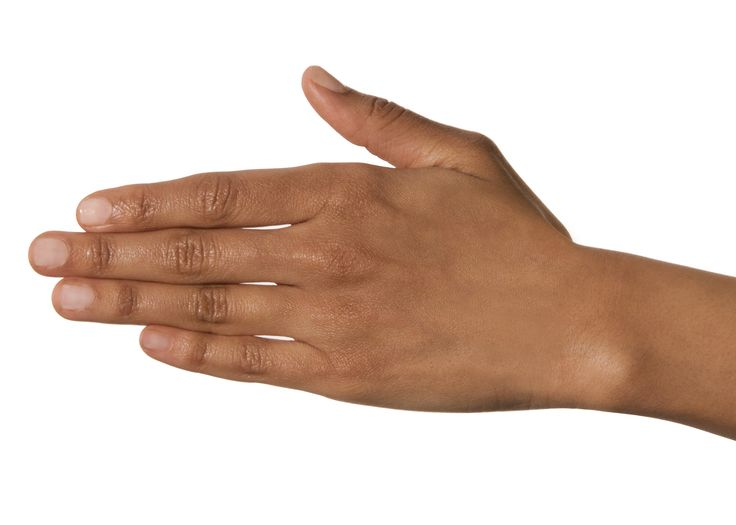
\includegraphics[width=\textwidth,height=\textheight,keepaspectratio]{../inputs/hand_brown.jpg}
  \end{minipage} & 
  \begin{minipage}{.29\textwidth}
    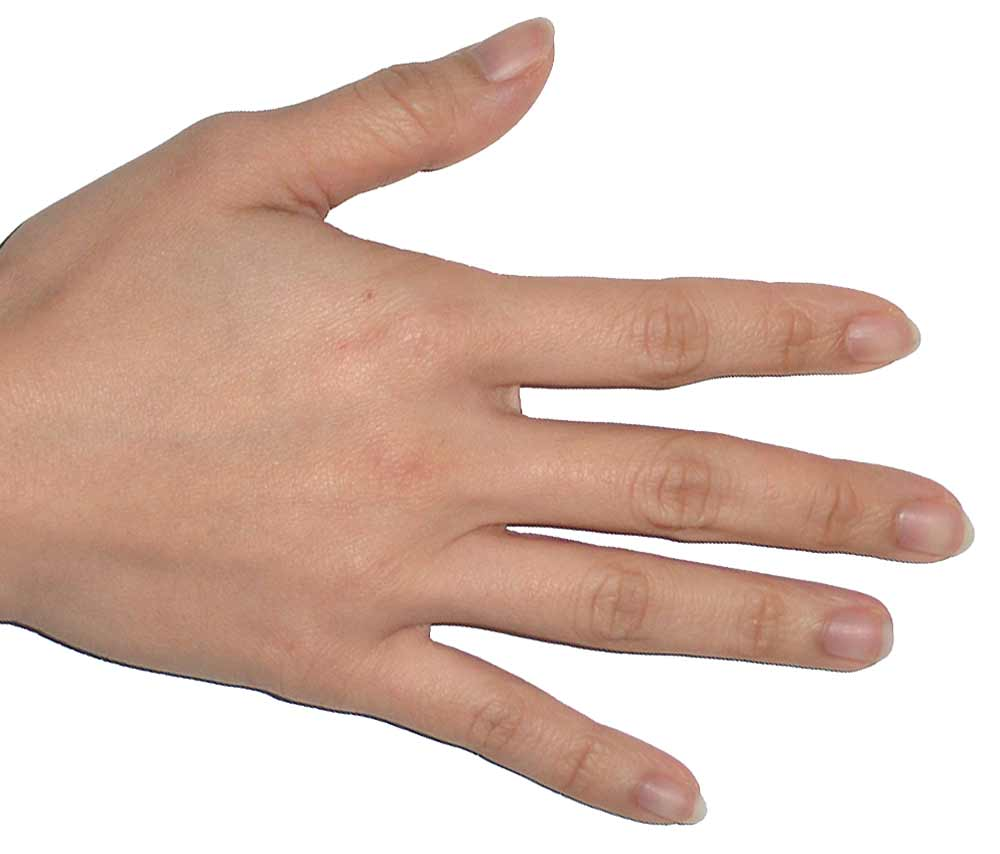
\includegraphics[width=\textwidth,height=\textheight,keepaspectratio]{../inputs/hand_light.jpg}
  \end{minipage} & 
  \begin{minipage}{.29\textwidth}
    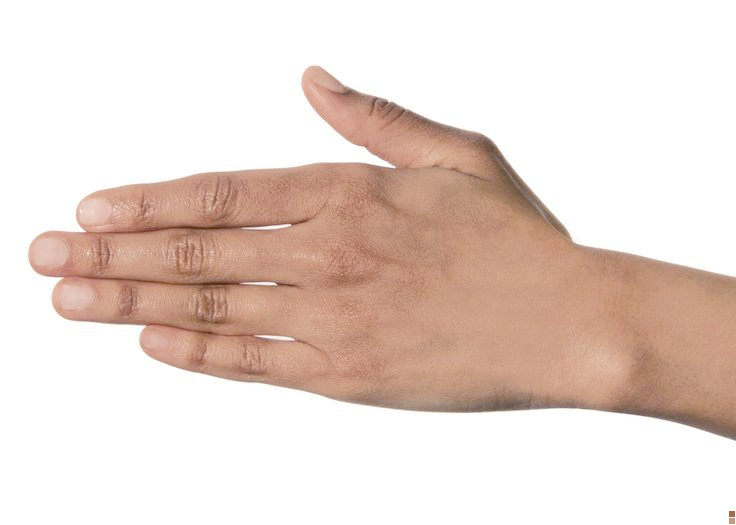
\includegraphics[width=\textwidth,height=\textheight,keepaspectratio]{../rc_test/outputs/20170516_proportional_test/hand_brown_to_hand_light.jpg}
  \end{minipage} \\
\hline  \label{row:prop_test_1} &
  \begin{minipage}{.29\textwidth}
    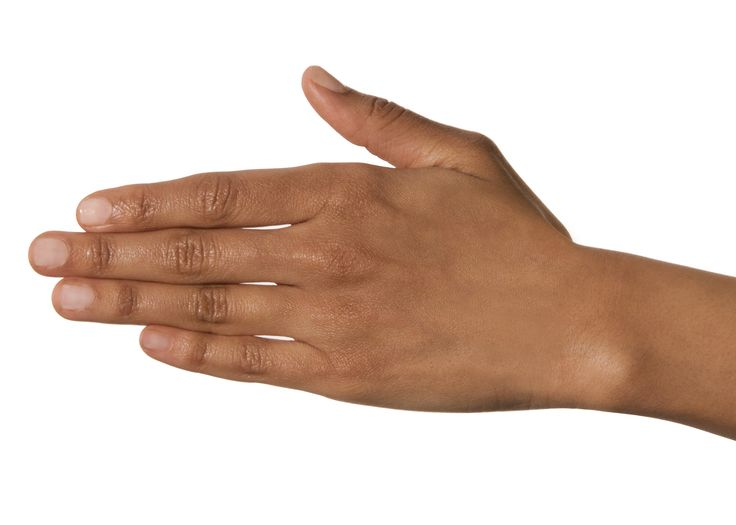
\includegraphics[width=\textwidth,height=\textheight,keepaspectratio]{../inputs/hand_brown.jpg}
  \end{minipage} & 
  \begin{minipage}{.29\textwidth}
    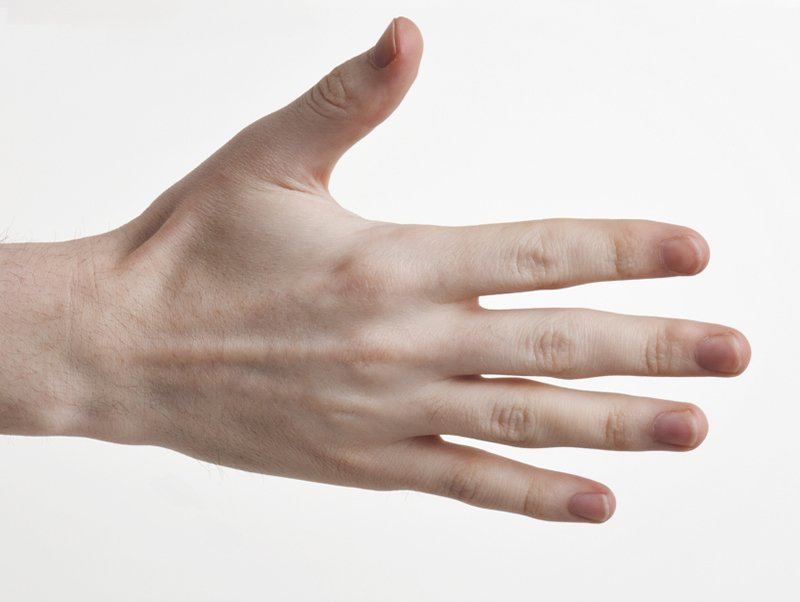
\includegraphics[width=\textwidth,height=\textheight,keepaspectratio]{../inputs/hand_pale.jpg}
  \end{minipage} & 
  \begin{minipage}{.29\textwidth}
    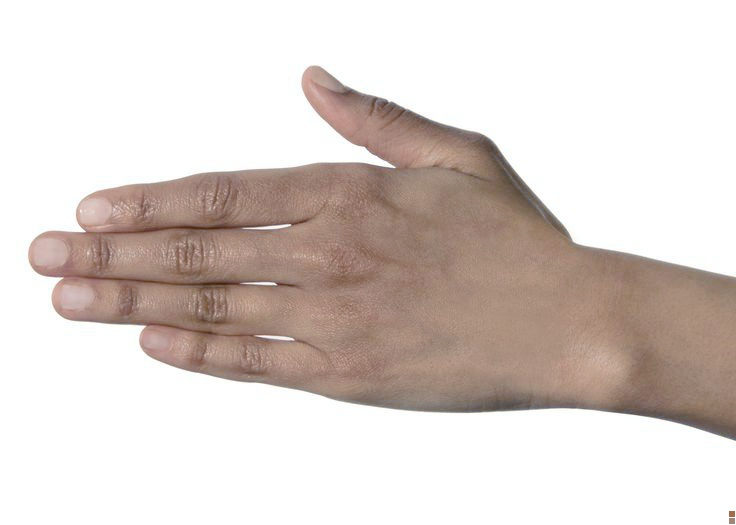
\includegraphics[width=\textwidth,height=\textheight,keepaspectratio]{../rc_test/outputs/20170516_proportional_test/hand_brown_to_hand_pale.jpg}
  \end{minipage} \\
\hline  \label{row:prop_test_1} &
  \begin{minipage}{.29\textwidth}
    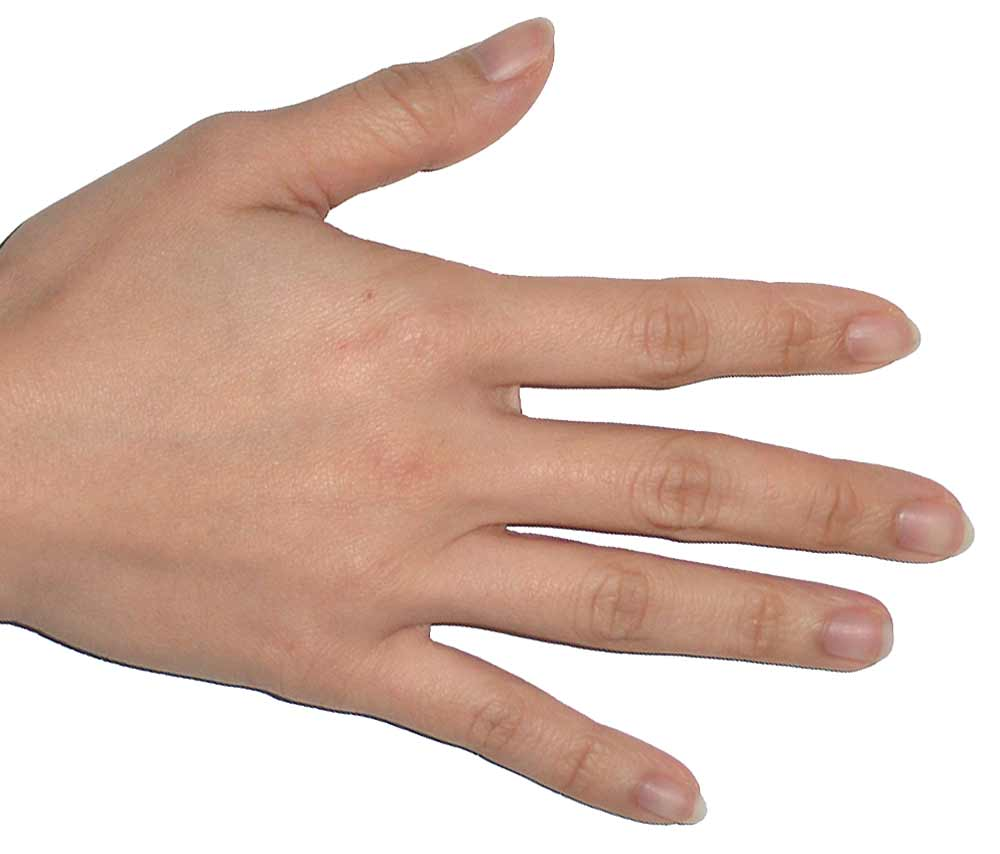
\includegraphics[width=\textwidth,height=\textheight,keepaspectratio]{../inputs/hand_light.jpg}
  \end{minipage} & 
  \begin{minipage}{.29\textwidth}
    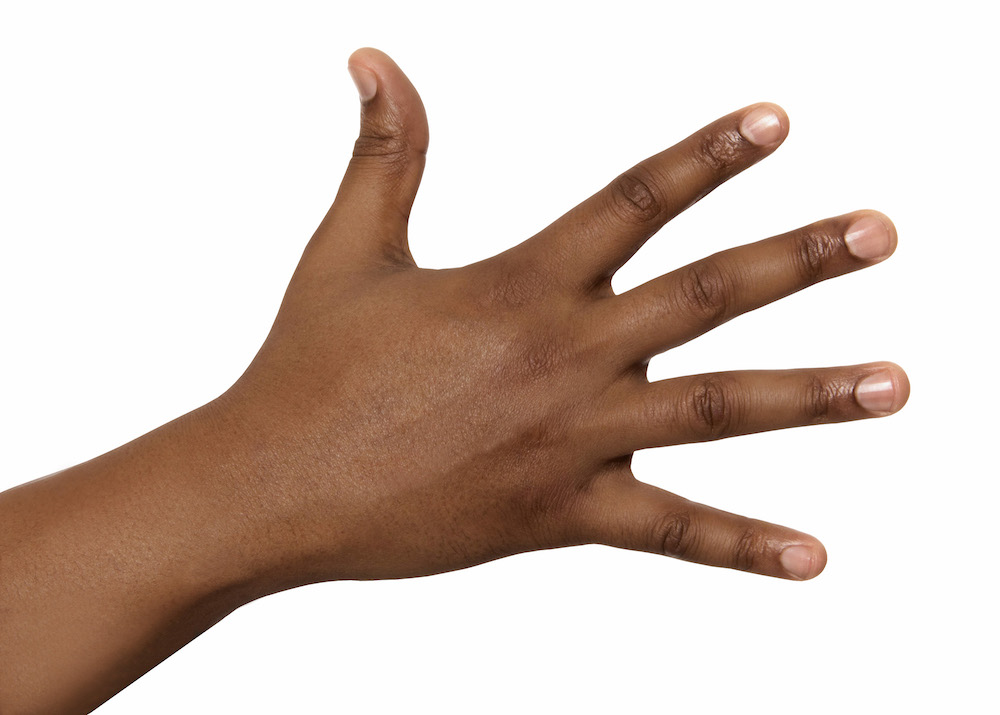
\includegraphics[width=\textwidth,height=\textheight,keepaspectratio]{../inputs/hand_dark.jpg}
  \end{minipage} & 
  \begin{minipage}{.29\textwidth}
    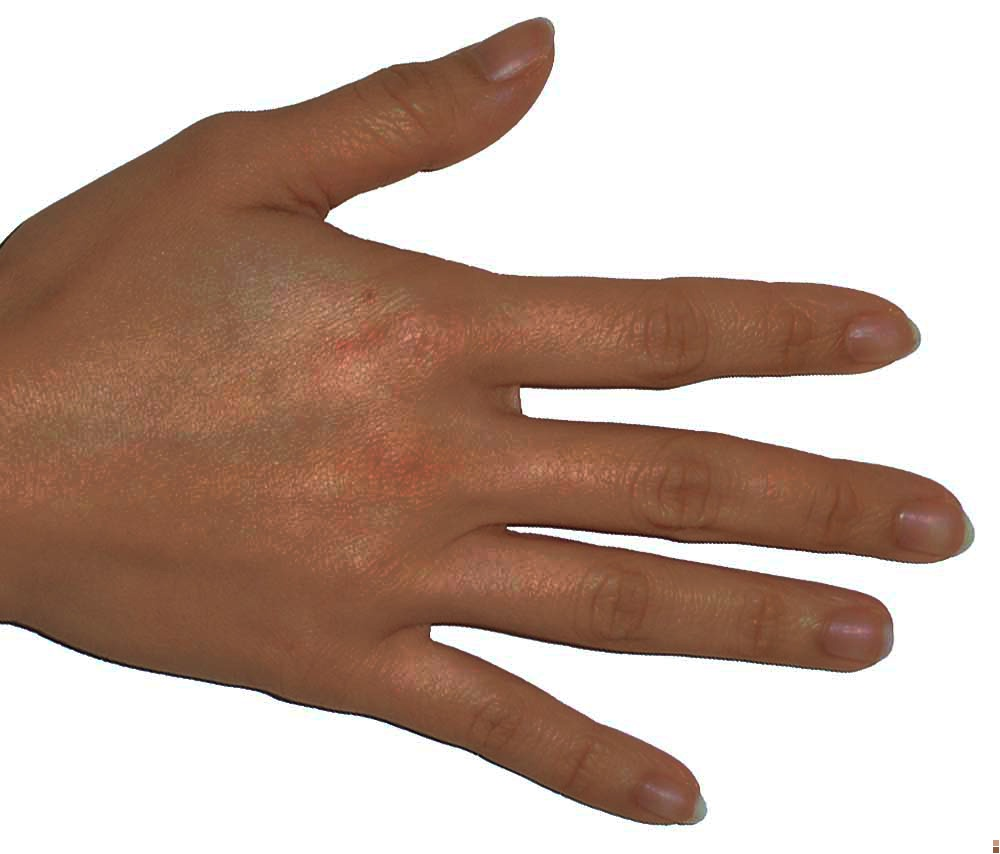
\includegraphics[width=\textwidth,height=\textheight,keepaspectratio]{../rc_test/outputs/20170516_proportional_test/hand_light_to_hand_dark.jpg}
  \end{minipage} \\
\hline  \label{row:prop_test_1} &
  \begin{minipage}{.29\textwidth}
    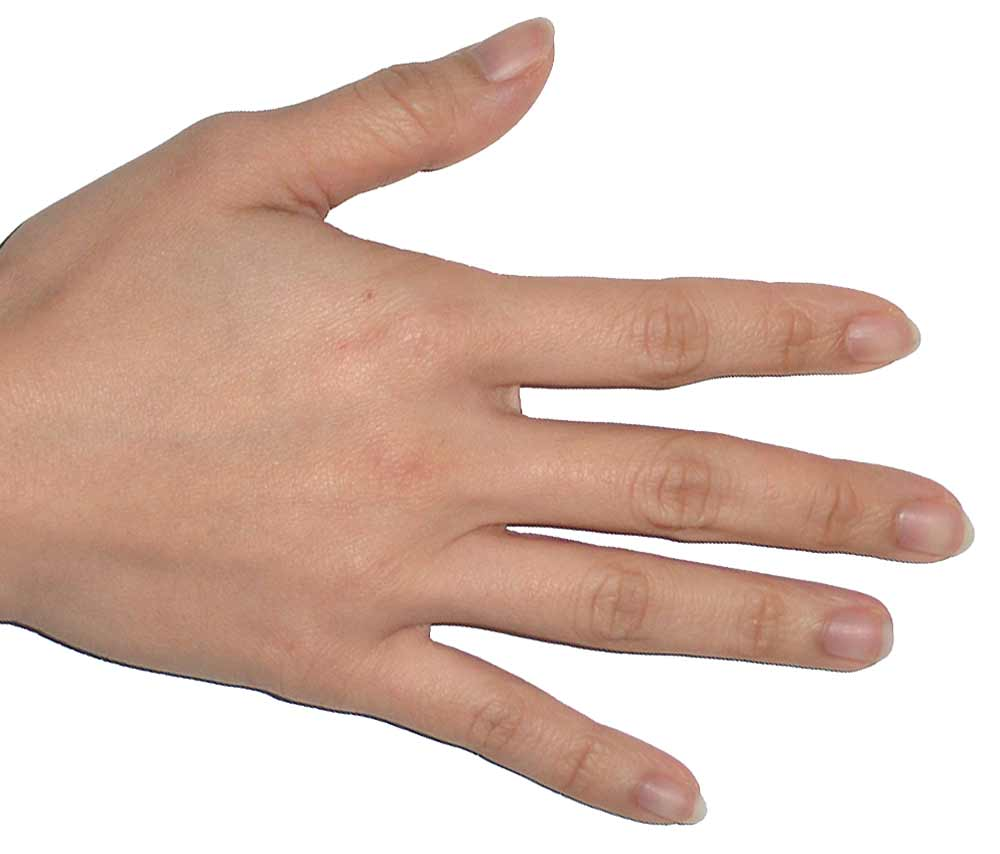
\includegraphics[width=\textwidth,height=\textheight,keepaspectratio]{../inputs/hand_light.jpg}
  \end{minipage} & 
  \begin{minipage}{.29\textwidth}
    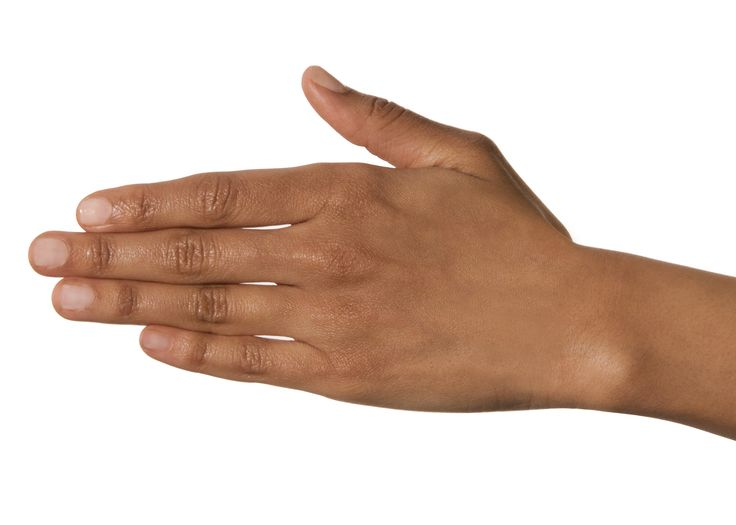
\includegraphics[width=\textwidth,height=\textheight,keepaspectratio]{../inputs/hand_brown.jpg}
  \end{minipage} & 
  \begin{minipage}{.29\textwidth}
    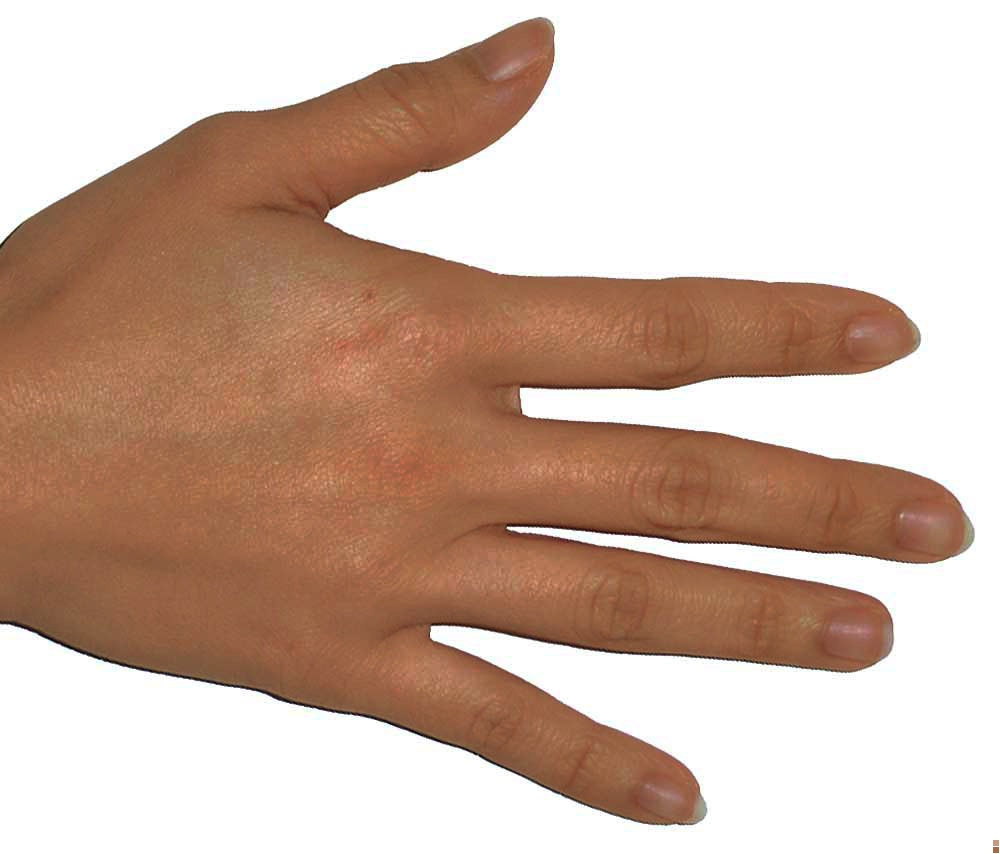
\includegraphics[width=\textwidth,height=\textheight,keepaspectratio]{../rc_test/outputs/20170516_proportional_test/hand_light_to_hand_brown.jpg}
  \end{minipage} \\
\hline  \label{row:prop_test_1} &
  \begin{minipage}{.29\textwidth}
    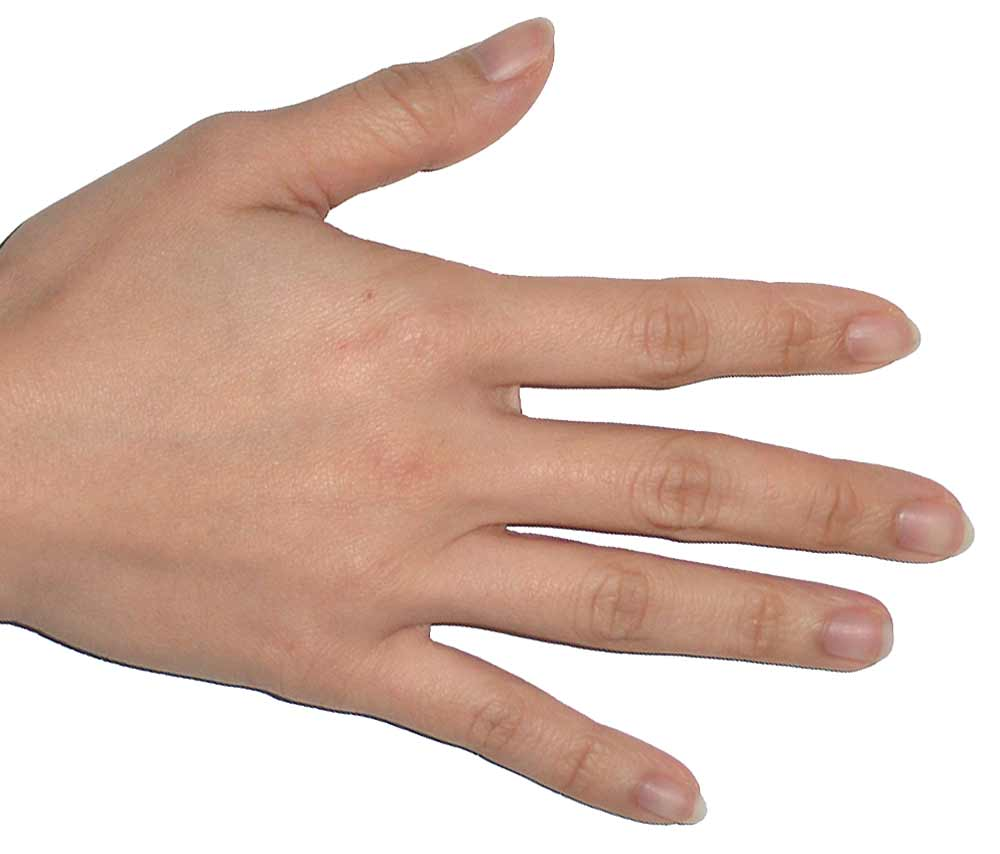
\includegraphics[width=\textwidth,height=\textheight,keepaspectratio]{../inputs/hand_light.jpg}
  \end{minipage} & 
  \begin{minipage}{.29\textwidth}
    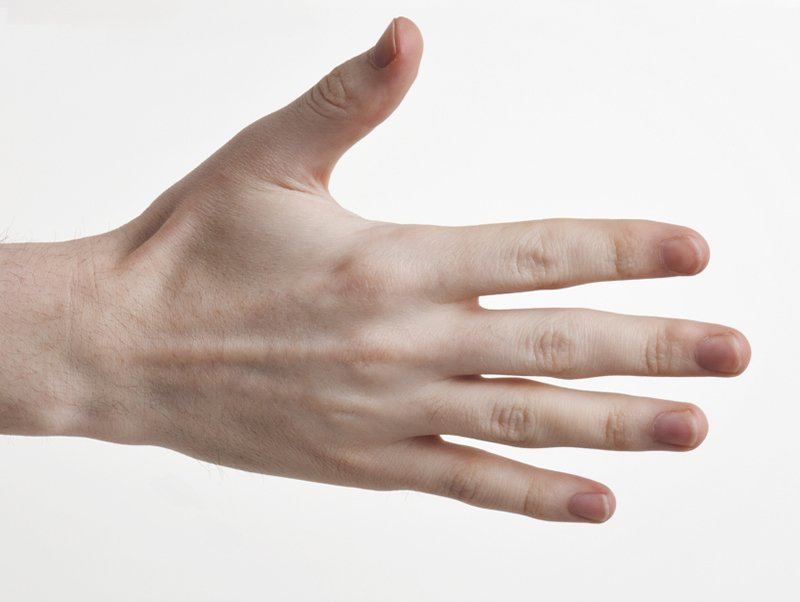
\includegraphics[width=\textwidth,height=\textheight,keepaspectratio]{../inputs/hand_pale.jpg}
  \end{minipage} & 
  \begin{minipage}{.29\textwidth}
    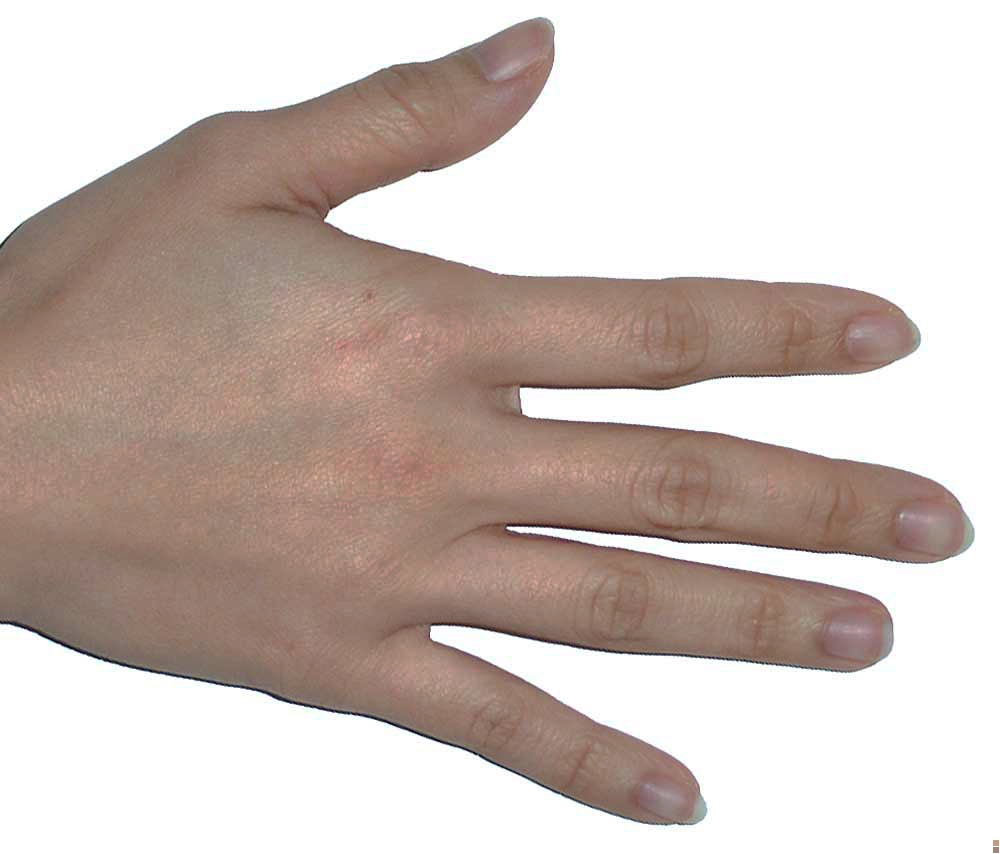
\includegraphics[width=\textwidth,height=\textheight,keepaspectratio]{../rc_test/outputs/20170516_proportional_test/hand_light_to_hand_pale.jpg}
  \end{minipage} \\
\hline  \label{row:prop_test_1} &
  \begin{minipage}{.29\textwidth}
    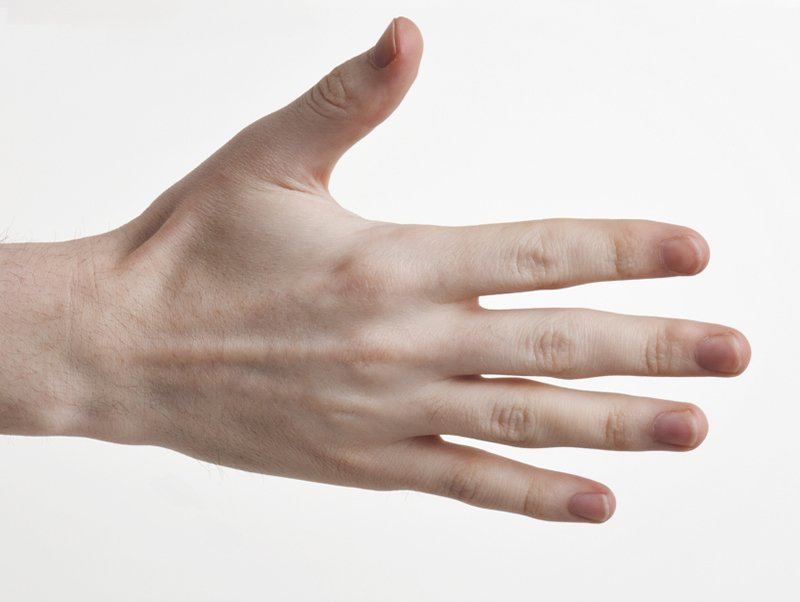
\includegraphics[width=\textwidth,height=\textheight,keepaspectratio]{../inputs/hand_pale.jpg}
  \end{minipage} & 
  \begin{minipage}{.29\textwidth}
    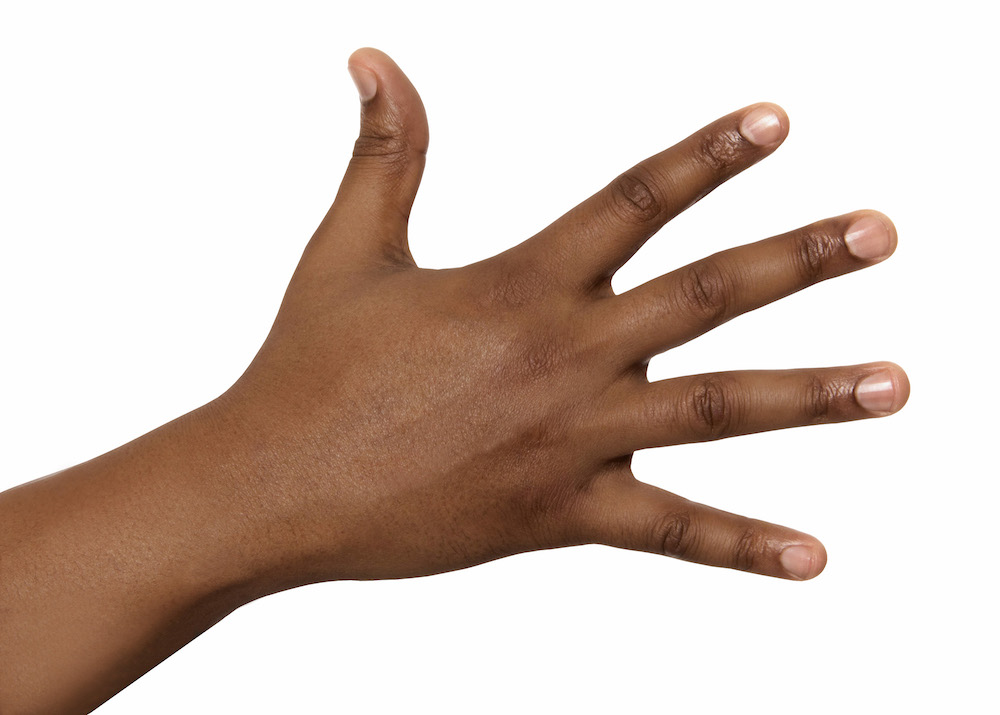
\includegraphics[width=\textwidth,height=\textheight,keepaspectratio]{../inputs/hand_dark.jpg}
  \end{minipage} & 
  \begin{minipage}{.29\textwidth}
    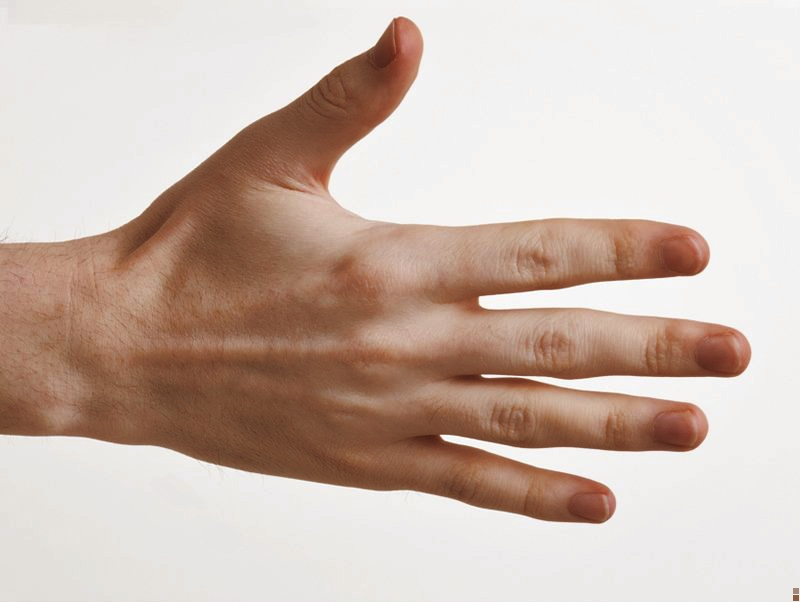
\includegraphics[width=\textwidth,height=\textheight,keepaspectratio]{../rc_test/outputs/20170516_proportional_test/hand_pale_to_hand_dark.jpg}
  \end{minipage} \\
\hline  \label{row:prop_test_1} &
  \begin{minipage}{.29\textwidth}
    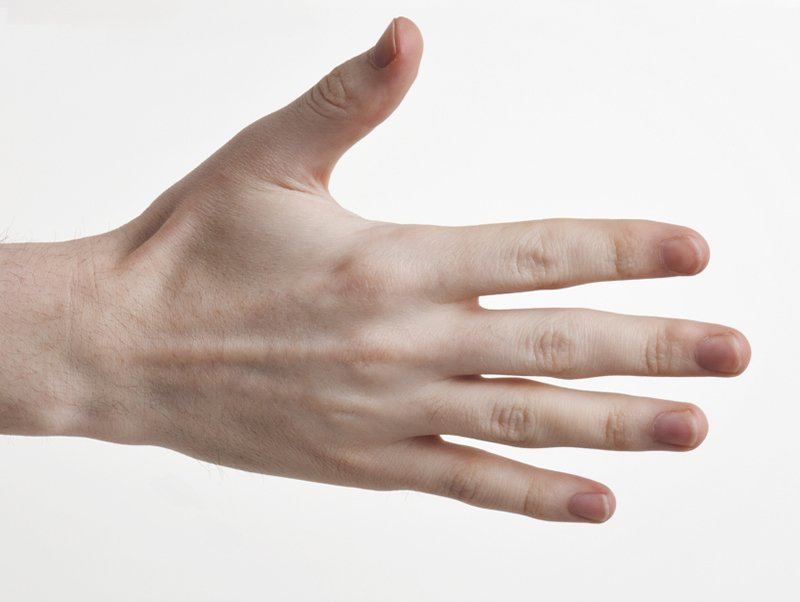
\includegraphics[width=\textwidth,height=\textheight,keepaspectratio]{../inputs/hand_pale.jpg}
  \end{minipage} & 
  \begin{minipage}{.29\textwidth}
    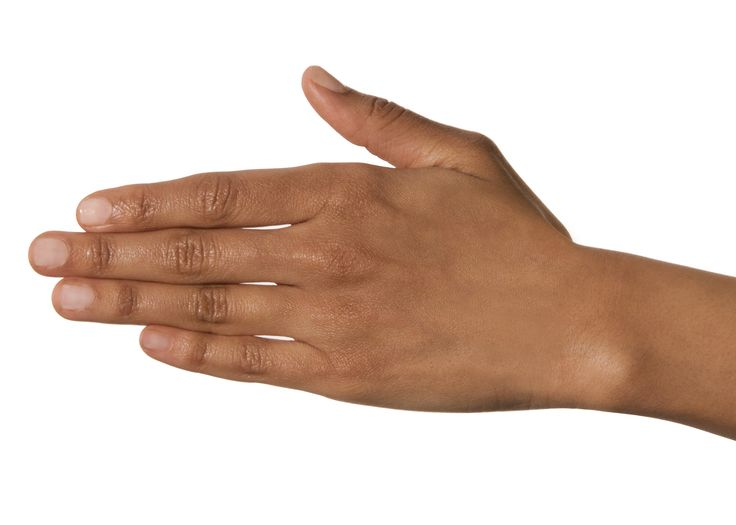
\includegraphics[width=\textwidth,height=\textheight,keepaspectratio]{../inputs/hand_brown.jpg}
  \end{minipage} & 
  \begin{minipage}{.29\textwidth}
    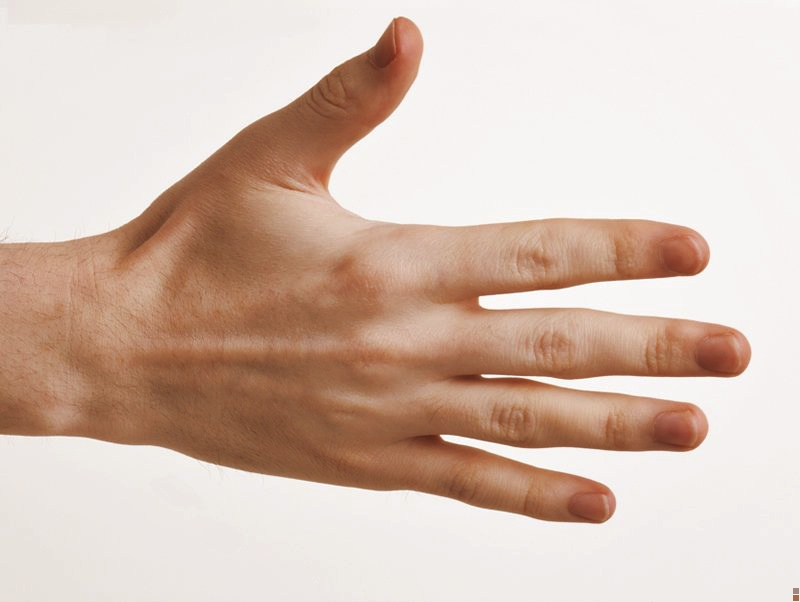
\includegraphics[width=\textwidth,height=\textheight,keepaspectratio]{../rc_test/outputs/20170516_proportional_test/hand_pale_to_hand_brown.jpg}
  \end{minipage} \\
\hline  \label{row:prop_test_1} &
  \begin{minipage}{.29\textwidth}
    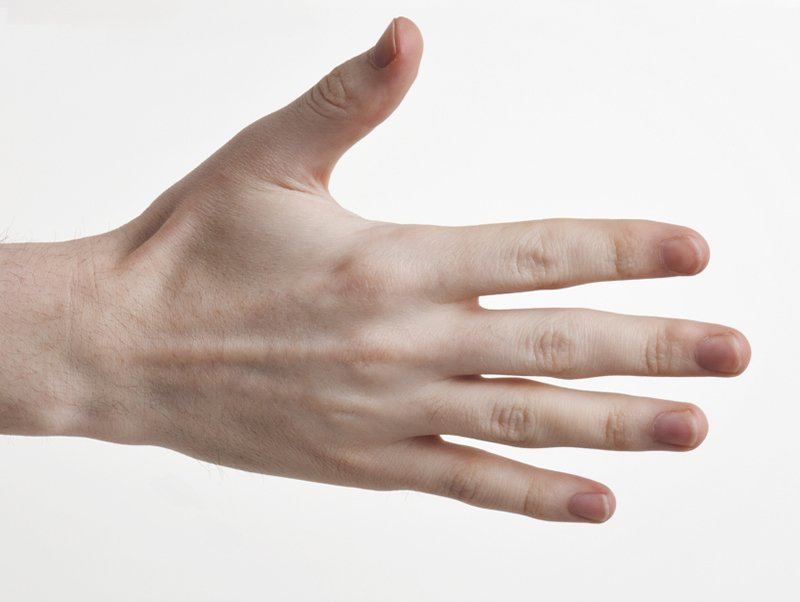
\includegraphics[width=\textwidth,height=\textheight,keepaspectratio]{../inputs/hand_pale.jpg}
  \end{minipage} & 
  \begin{minipage}{.29\textwidth}
    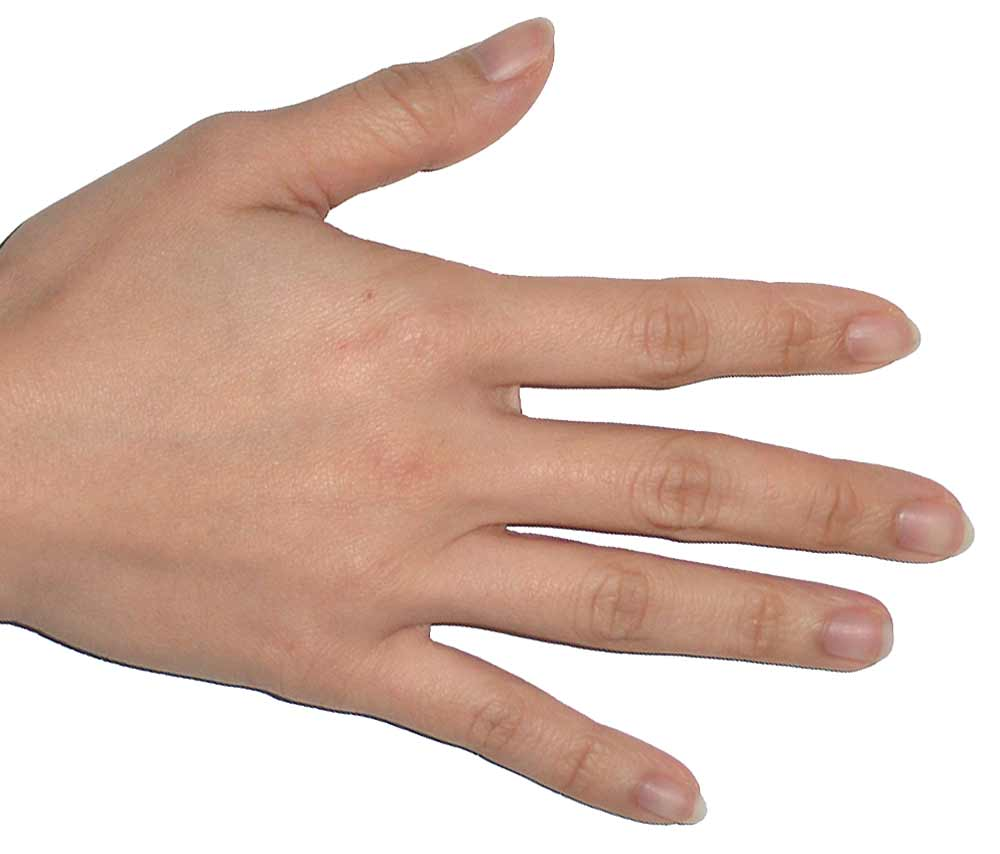
\includegraphics[width=\textwidth,height=\textheight,keepaspectratio]{../inputs/hand_light.jpg}
  \end{minipage} & 
  \begin{minipage}{.29\textwidth}
    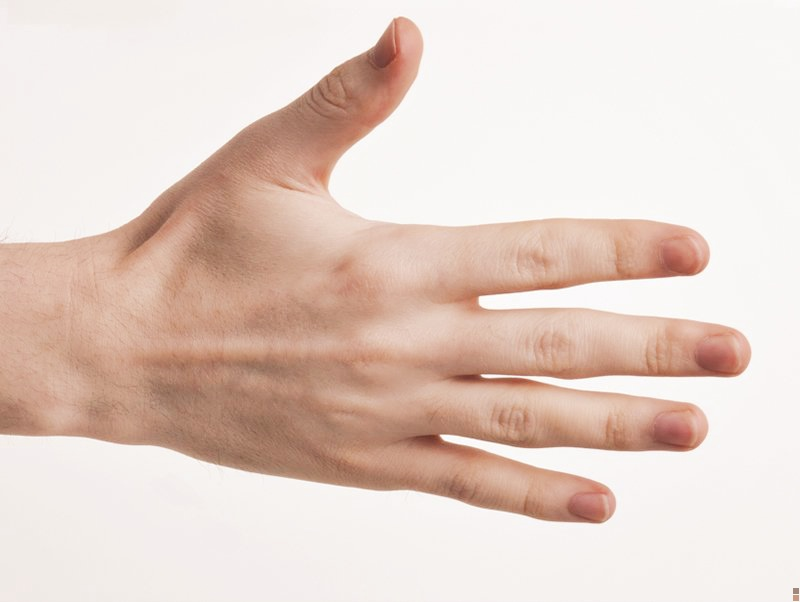
\includegraphics[width=\textwidth,height=\textheight,keepaspectratio]{../rc_test/outputs/20170516_proportional_test/hand_pale_to_hand_light.jpg}
  \end{minipage} \\
\hline
 \end{longtable}

This method improved the appearance of cases with over-bright spots or ``high-key" appearance issues, as Figure \ref{img:compare_bright_spot} shows:
\begin{figure}[H]
    \centering
    \begin{subfigure}[b]{0.40\textwidth}
        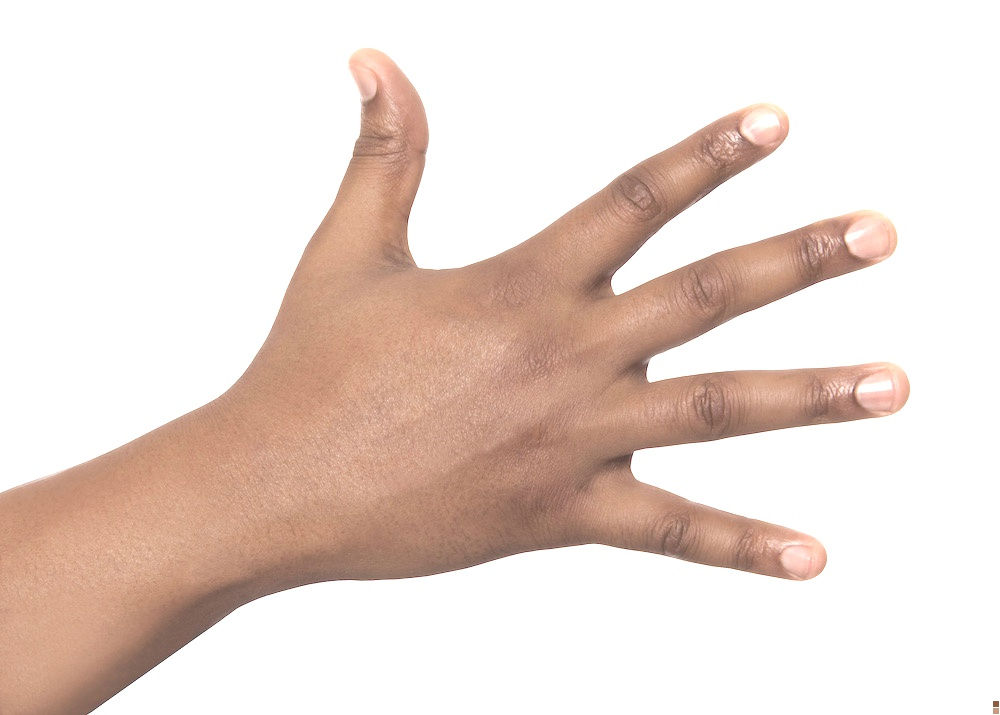
\includegraphics[width=\textwidth]{../rc_test/outputs/20170516_boost_test/hand_dark_to_hand_light.jpg}
        \caption{Simple addition algorithm (Equation \ref{eq:boost_algo})result}
    \end{subfigure}
    ~
    \begin{subfigure}[b]{0.40\textwidth}
        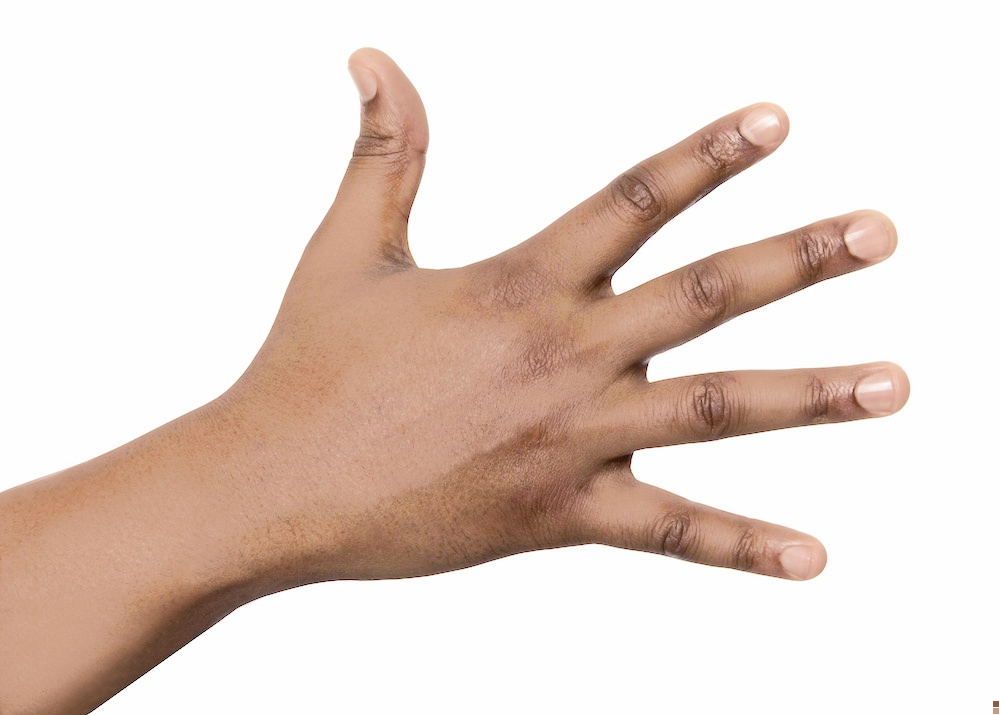
\includegraphics[width=\textwidth]{../rc_test/outputs/20170516_proportional_test/hand_dark_to_hand_light.jpg}
        \caption{Proportional adjustment algorithm (Equation \ref{eq:prop_algo}) result}
    \end{subfigure}
    \caption{Comparison of algorithms \ref{eq:boost_algo} and \ref{eq:prop_algo} results for transforming a dark hand (Figure \ref{img:input_hands_1_dark}) to a light hand (Figure \ref{img:input_hands_1_light}).\label{img:compare_bright_spot}}
\end{figure}

We noted however, that this method noticeably does not correct for, and even exacerbates slightly relative to the simple addition algorithm the dark spots at the joints and creases of a hand of darker skin tone when it is transformed to a lighter skin tone (Row \ref{row:prop_test_hand_brown_to_hand_light}). Other results are similar to the results of the simple addition algorithm.
